\documentclass[journal]{IEEEtran}
\usepackage{amsmath,amsfonts}
\usepackage{algpseudocode}
\usepackage{algorithm}
\usepackage{array}
\usepackage[caption=false,font=normalsize,labelfont=sf,textfont=sf]{subfig}
\usepackage{caption}
\usepackage{textcomp}
\usepackage{stfloats}
\usepackage{url}
\usepackage{verbatim}
\usepackage{graphicx}
\usepackage{cite}
\usepackage{color, soul}
\usepackage{hyperref}
\usepackage{listings}
\hyphenation{op-tical net-works semi-conduc-tor IEEE-Xplore}

\lstset{
  basicstyle        = \ttfamily,
  captionpos        = b,
  columns           = fullflexible,
  breaklines        = true,
  postbreak         = \mbox{\textcolor{blue}{$\hookrightarrow$}\space},
}

\newcommand{\italic}[1]{{\textit{#1}}}

\begin{document}

\title{Can an Unknowing Participant distinguish between Multi-Agent Designed and Human Designed Interiors?}

\author{Thomas O'Leary}

\maketitle

% Abstract
\begin{abstract}

What's the problem? What am I looking at? How does that help solve the problem?
\\
\\
Opening, Challenge, Action, Resolution
\\
\\
Attempt to see if procedural generated interiors can be percieved as human designed. Comparing the two together and see if participants prefer the procedurally generated designs.

\end{abstract}

% Introduction
\section{Introduction}

Urban open world games such as the Grand Theft Auto series[cite], The Division series[cite] and the Batman Arkham series[cite]
have such large built-up areas for players to venture in, but many buildings are blocked off - 
if you're lucky to have access to a building you are still very limited to the rooms you are able to enter.
Possibly ruining the immersion of the game for players.

This problem could be fixed by having developers designing each and every room in every single building within the vast urban environment.
But this would become a very time-consuming and impractical task.

Using Procedural Generation (PCG), this largely time-consuming task of designing room interiors can be automated. And can possibly help maintain a player's immersion within the game.

An issue with this however is that PCG tool's can be seen as boring and repetitive \cite{pcg_in_gd} 

Through my literature review though I have found many implementations and techniques of Procedural Interior Generation (PCIG), none of these get compared to Human designed interiors. 

This study looks to see if a participant is able to tell the difference between Human designed and AI generated interiors.

%urban open world games such as the Grand Theft Auto series, Watchdogs series and the Batman Arkham series
%have such large built-up urban areas for players to venture in but many buildings/rooms inside buildings are blocked off, stopping players from exploring inside.

%Assassins Creed Unity

%simply, designers could model these interiors by themselves but due to the ever increasing nature of open world games - this would become and already is impractical and very time consuming/

%using procedural generation techniques, this time consuming task can be automated to allow designers to focus on other things blah blah blah

%the issue at hand is procedural generation can tend to be repetitive, dull and could potentially ruin the emersion of a game.

%this study looks to see if someone is able to tell the difference between hand made and AI generated interiors.


% Literature Review    
\section{Literature Review}
\hl{My literature review consists of two parts that I believe to be important to my research question. It first describes different implementations of Procedural Interior Generation (PCIG) then explores ways in which Artificial Intelligence (AI) is compared to Humans.}

\subsection{Implementations of Procedural Interior Generation}
Although PCG has a lot to show and offer in game development \hl{- being used for characters, terrain, and textures -} the use of Procedural Interior Generation (PCIG) in games however is scarcely come by.
\\
A game that does use PCIG is Catlateral Damage \cite{game:catlateral},
a small indie game developed by Manekoware where you play as a cat on a destructive rampage 
in its own house. In 2017, Chris Chung (the developer behind the game) wrote a case study about the level design in his game \cite[Chapter~6]{what-is-pcg}. When developing Catlateral Damage, Chung was undecided on how to design the levels and ultimately went for PCIG\cite{pcg_in_gd}. Before the interior decoration can take place, a Squarified Treemap algorithm is used to generate the room layouts and floor plans within the level \cite{squarified-treemap}. Each room generated from this algorithm has an associated data file, this file contains data such as furniture available and maximum type of each furniture. The furniture objects that can be placed have physics components attached, to allow them to be accurately placed within the level - for this, a Rectangle Packing algorithm is used to place these objects within allocated surface areas on the floor and other furniture objects. Concluding the case study, Chung states that most players could not notice that the levels were procedurally generated - \hl{although this is a promising statement, Chung has not shown any evidence to back this claim.}
\\
On 29th April 2021, Sony Interactive Entertainment published patent US20210121781, titled "AI-Generated Internal Environments Based On External Geometry" \cite{sony-patent}. The patents' description goes onto explain a Machine Learning (ML) tool that takes in data from the external structure of a virtual building and generates an interior environment just from this data. \hl{Although this is just a patent for an ML tool, this could be the start of PCIG being used in AAA Titles. }
\bigskip


Despite there not being many implementations of PCIG in games, there are however a handful of published papers that have used their own techniques to emulate room interiors.
\subsubsection*{Multi-Agent System}
In 2009, T. Germer and M.Schwarz sought out to procedurally arrange a rooms' furniture in real-time. \cite{real-time-walkthroughs}. A demonstration of this system can be found on YouTube, uploaded by T. Germer himself \cite{youtube:real-time-walkthroughs}. This system involves a Multi-Agent based solution where each furniture object, in a given room, is seen as an individual agent that seeks a suitable parent furniture object. These agents have custom semantic descriptions to allow them to create different object layouts, an example listed by the authors is a chair - a chair can either be set next to a table/desk but can also be isolated in its own surroundings leading it to have many possible parent objects \cite{real-time-walkthroughs}.\\
Each agent has 3 states:
\begin{enumerate}
    \item Search
        \begin{itemize}
            \item All agents start in this state, they begin by searching for possible parent objects - if a parent is found that suits its semantics the agents' state changes to \textit{Arrange}, if a parent can't be found at all the agent is deleted. Different parts of the room are set as the root parent for agents - floor, walls, windows and doors.
        \end{itemize}
    \item Arrange
        \begin{itemize}
            \item In the \textit{Arrange} state, the agent attempts to place and orient itself with the parent accordingly. Whilst doing so, it has to check for collisions with other agents in which the Separating Axis Thereom is used \cite{separating-axis-thereom} - if no collisions are found the agents' state changes to \textit{Rest}.
        \end{itemize}
    \item Rest
        \begin{itemize}
            \item In the \textit{Rest} state, potential child agents are now able to seek this object as a parent. If the resting agents parent moves, the resting agent will move along with it - however if this move results in a collision, its parent is lost and the agents state is changed back to \textit{Search}.
        \end{itemize}
\end{enumerate}
Before using this system, it requires a certain degree of user input \cite{real-time-walkthroughs}. Firstly, each room would need to have specific data such as labelled parts of the room (windows, floor, doors), how many objects, what type of objects and how many of these types can be used in this room.
A user is also required to write the semantic description of each type of object - this includes object clearance distance, possible orientation values and potential parents (and what sides to correspond with).
Due to the parents of each object being manually set by the user in their semantic descriptions, a hierarchy is not explicitly defined - yet handled at run-time by the system just before the agents are initialised \cite{real-time-walkthroughs}.

\hl{Although a large proportion of the rooms furnishing is handled by the agents themselves, a big drawback is that each agent must have a manually defined semantic description. This could cause a lot of issues especially if many types of objects are to be used in a room.}

\subsubsection*{Rule-Based Layout}
A Rule-Based layout approach was proposed in 2009, this method would focus on user defined rules and layouts \cite{rule-based-layout}. Users would be able to specify what objects can be placed within a layout - these would represent an instance of a class and contain certain rules on how it should behave when being placed.

The relationships between different objects could be explicitly and implicitly defined. A user is able to explicitly create a rule in an objects class or use features. An example of explicitly defining a relationship, as told by the authors, is by setting rule for the sofa class to always face an instance of the TV class \cite{rule-based-layout}.
An implicitly defined relationship uses feature types. Feature types can be used for checking what objects should and should not overlap. These are used as tags and are applied to specific parts of objects - for example an \textit{OffLimit} feature type tag would be used for the bounding box of most objects \cite{rule-based-layout}.

Rules can be defined in multiple ways too. They can be associated specifically with an object class, this would mean that this rule only applies to this class and any instances of it.
Another way is by defining rules in the layout planner - this would help with objects that general rules may not be applicable to. An example listed by the authors is a chair in a meeting room, this type of object is usually sat against a wall - so this rule would be applied in a "Waiting Room" layout \cite{rule-based-layout}.

The layout planner is responsible for sending objects to the layout solver. As stated before, the planner can have custom rules itself to allow it to be applicable to different room layouts (living room, factory floor, waiting room). It also has a backtracking rule that is only triggered if an object of interest is not placeable. If this is the case, the planner would backtrack to place previous objects in different positions to allow this object to be placed.

The layout solver is given an object from the planner and the type of layout (dependent if a user has applied rules to the planner). Within this layout it finds all possible locations for the new object - these possible locations are initially based upon the set rules of the object and the rules already set in place for existing objects in the layout. The possible locations then take into account specific feature types, such as the amount of clearance an object requires or the \textit{OffLimit} tag that was mentioned earlier \cite{rule-based-layout}. A Minkowski Sum \cite{minkowski} is carried out containing these inaccessible areas and removed from the list of possible locations.
With this completed, the object is then given a list of all possible locations in the layout it can be placed.

\hl{Something good. Something bad.}

\subsubsection*{Constraints}
In 2017 P. Henderson, K. Subr and V. Ferrari presented a data driven model that learns from the SUNCG \cite{suncg} database to generate furniture layouts \cite{constrained-layouts}. This database contains over 45000 apartment layouts that are designed by humans, from this 45000 - 2500 CAD models are categorised into furniture, these models are then assigned an object class of which there is 170 of (television, bed, table).
Their model is presented in such a way that it can be left to be fully automated \cite{constrained-layouts}, but does allow flexibility with the user allowing them to change constraints within the layout.\\
These constraints include:
\begin{itemize}
    \item Room size, shape \& type 
    \item Exclusion of Object classes
    \item Furniture clearance 
    \item Locations of specified furniture
    \item Locations of doors \& windows
\end{itemize}
Upon generating layouts, the results varied dependent on the set constraints applied to the room. Layouts that had no set constraints were found to be generating in 0.04 seconds on average \cite{constrained-layouts}. Whereas layouts that did have constraints applied, generated anywhere between 0.04-112 seconds on average \cite{constrained-layouts}. This large difference in generation times drastically varies solely on what constraints applied -  room size, object exclusion and clearance constraints all generated in 0.04 seconds on average, whereas the combination of room size and the locations of doors \& windows took around 112 seconds to generate.

A user study was carried out in their paper, where 1400 pairs of layouts are presented to 8 non-experts in an image format \cite{constrained-layouts}. These participants are asked to identify the layout that has a more realistic/natural setting. In each pair one layout is from their model, the other being human designed - the order in which these images are shown are randomised per pair.
In this study, both constrained and unconstrained layouts are put to the test. For unconstrained layouts, they were presented in 2 different styles; 1st person and an overhead view. Layouts that were presented in 1st person, were seen to be slightly preferred over the human designs and those presented overhead were seen to be indistinguishable from human designs.
Constrained layouts were only presented in an overhead format, but two sets of constraints were used:
\begin{enumerate}
    \item[i.] Fixed room size \& fixed placement of a singular object
    \item[ii.] Fixed room size \& fixed door/window locations
\end{enumerate}
With the constrained layouts of (i), the model layouts were seen to be indistinguishable from those of human design. Whereas the layouts of (ii), human designs were preferred over the models.

\hl{Something good. Something user study. Something bad.}

\subsubsection*{Statistical Relationships}
Paper \cite{make-it-home}
YouTube video \cite{youtube:make-it-home}
Simulated annealing \cite[Chapter~3]{simulated-annealing}
M-H algorithm \cite{understanding-mh-algorithm}

\subsection{Artificial Intelligence Compared to Humans}
This is going to be a little more difficult to write about, as I haven't read a paper on this so far. And I have only managed to find 3 papers that talk about this, but I am not sure that they could be entirely relevant.

% Research Question
\section{Research Question \& Artefact}
Through my literature review, there is evidence to show that PCIG should be compared to human designs more frequently to test its authenticity. With this I propose the following research question; \textit{Can an Unknowing Participant distinguish between a Multi-Agent Designed and Human Designed Interiors?}

\subsection{Hypotheses}
\begin{enumerate}
    \item When unaware, the M-A System is picked more often than Human designed interiors by participants
        %\begin{itemize}
        %    \item \hl{\textit{Null}: When unaware, the M-A System is not picked more often than Human designed interiors by participants}
        %\end{itemize}
    \item When notified, the participant is not able to distinguish between human and M-A system interiors
        %\begin{itemize}
        %    \item \hl{\textit{Null}: When notified, the participant is able to distinguish between human and M-A system interiors by participants}
        %\end{itemize}
\end{enumerate}

\subsection{Artefact}
The artefact is a Multi-Agent (M-A) system that will be used to create a room's furniture arrangement where each furniture is seen as an individual agent. The system is given an empty room and has access to pre-made furniture assets, at run time agents are spawned and arrange themselves accordingly (the behavior of a singular agent is demonstrated in \hyperref[activity-diagram]{Fig. 1}). The artefact will be influenced by the work from \textit{T. Germer, et al.} \cite{real-time-walkthroughs}.

\subsection{How it will be made} 
The Unity game engine\cite{unity} will be used for the implementation of the artefact as I have a few years of experience in creating other projects within its environment also the knowledge I have in C\# and Unity's classes help towards choosing what engine I would prefer to use.
I will also be closely following the Agile Methodology and its principles to help with the development life cycle as Agile is commonly used in Software Engineering and Game Development environments alike \cite{game-dev-agile}.

\subsection{Quality Assurance} 
I plan to use C\#'s \textit{NUnit Framework} \cite{nunit-framework} for Unit testing to ensure my Artefact works as intended.


% Artefact
%\section{Artefact}

The artefact is a Multi-Agent (M-A) system that will be used to create a room's furniture arrangement where each furniture is seen as an individual agent. The system is given an empty room and has access to pre-made furniture assets, at run time agents are spawned and arrange themselves accordingly (the behavior of a singular agent is demonstrated in \hyperref[activity-diagram]{Fig. 1}). The artefact will be influenced by the work from \textit{T. Germer, et al.} \cite{real-time-walkthroughs}.

The Unity game engine will be used for the implementation \cite{unity} and I will also be following the Agile Methodology to help me with the development life cycle of the artefact.

%The system will involve using Unity's ScriptableObject class to hold the information about the furniture objects.

%\subsection{What will be made}
%A Multi-Agent (M-A) system that generates the interior of a room at run time. This room will have a pre-defined room size, the system will also have access to pre-made furniture assets.
%\hl{Something about using Real-Time walkthrough paper as an inspiration for the system}.

%\subsection{How will I create it}
%The AI will be made in the Unity game engine (Version 2020.3.12f1) \textbf{cite unity engine}

\subsection{How will I ensure Quality}
Unit tests \& Acceptance Tests?

\subsection{Why will this answer the Research Question}
The M-A system itself will not contribute towards answering the research question directly but will contribute towards the research study that will follow. 

%Long sentence that needs to be fixed LMAO
%\hl{This system will be used in my research to be compared with human designed interiors.}

% Research Methodology
\section{Research Methodology}

% NEED TO REWRITE THIS SECTION

\subsection{Experimental Design}
For my experimental design, a participant was shown 5 pairs of room layouts in the form of a 2 Staged A/B test.
In the first stage the participant was informed to pick, out of each pair, which room furniture layout they preferred. This preference may have been influenced by realism, authenticity or what environment they would rather be in. In each pair, one layout was that of human design and the other was designed by the Artefact (M-A System) - an example of this is shown in Fig~\ref{pair-example-1} \& Fig~\ref{pair-example-2}. The order in which these layouts were shown were randomised per stage and per participant.
Once 5 furniture arrangements were selected, the participant would move onto the second stage of the study - a notice would appear notifying the participant they have reached Stage 2, as shown in Fig~\ref{stage-2}. Just before beginning they were notified that in every pair within the first stage, 1 furniture layout was created by the Artefact (M-A System). Their challenge in the second stage of the study would be to select, out of the same 5 pairs they were initially shown, which one they believe was made by the Artefact (M-A System).

This experimental design was used as previous works by \italic{P. Henderson, et al.} \cite{constrained-layouts} and \italic{L.-F. Yu et al.} \cite{make-it-home} carried out similar perceptual studies requiring a participant to pick between one from their designed model and human designs. In 2010, Margaret Boden proposed a new variant of the Turing Test (TT) that is oriented around artistic creativity \cite{artistic-tt}. With her TT, for an art program to pass it would have to:
\begin{enumerate}
    \item Be indistinguishable from human produced artwork
    \item[]And/Or
    \item Be seen having similar aesthetic value to human produced artwork
\end{enumerate}
I found this variant of the TT as a helpful source when designing the experimental design for my research study.


\begin{figure}[!h]
    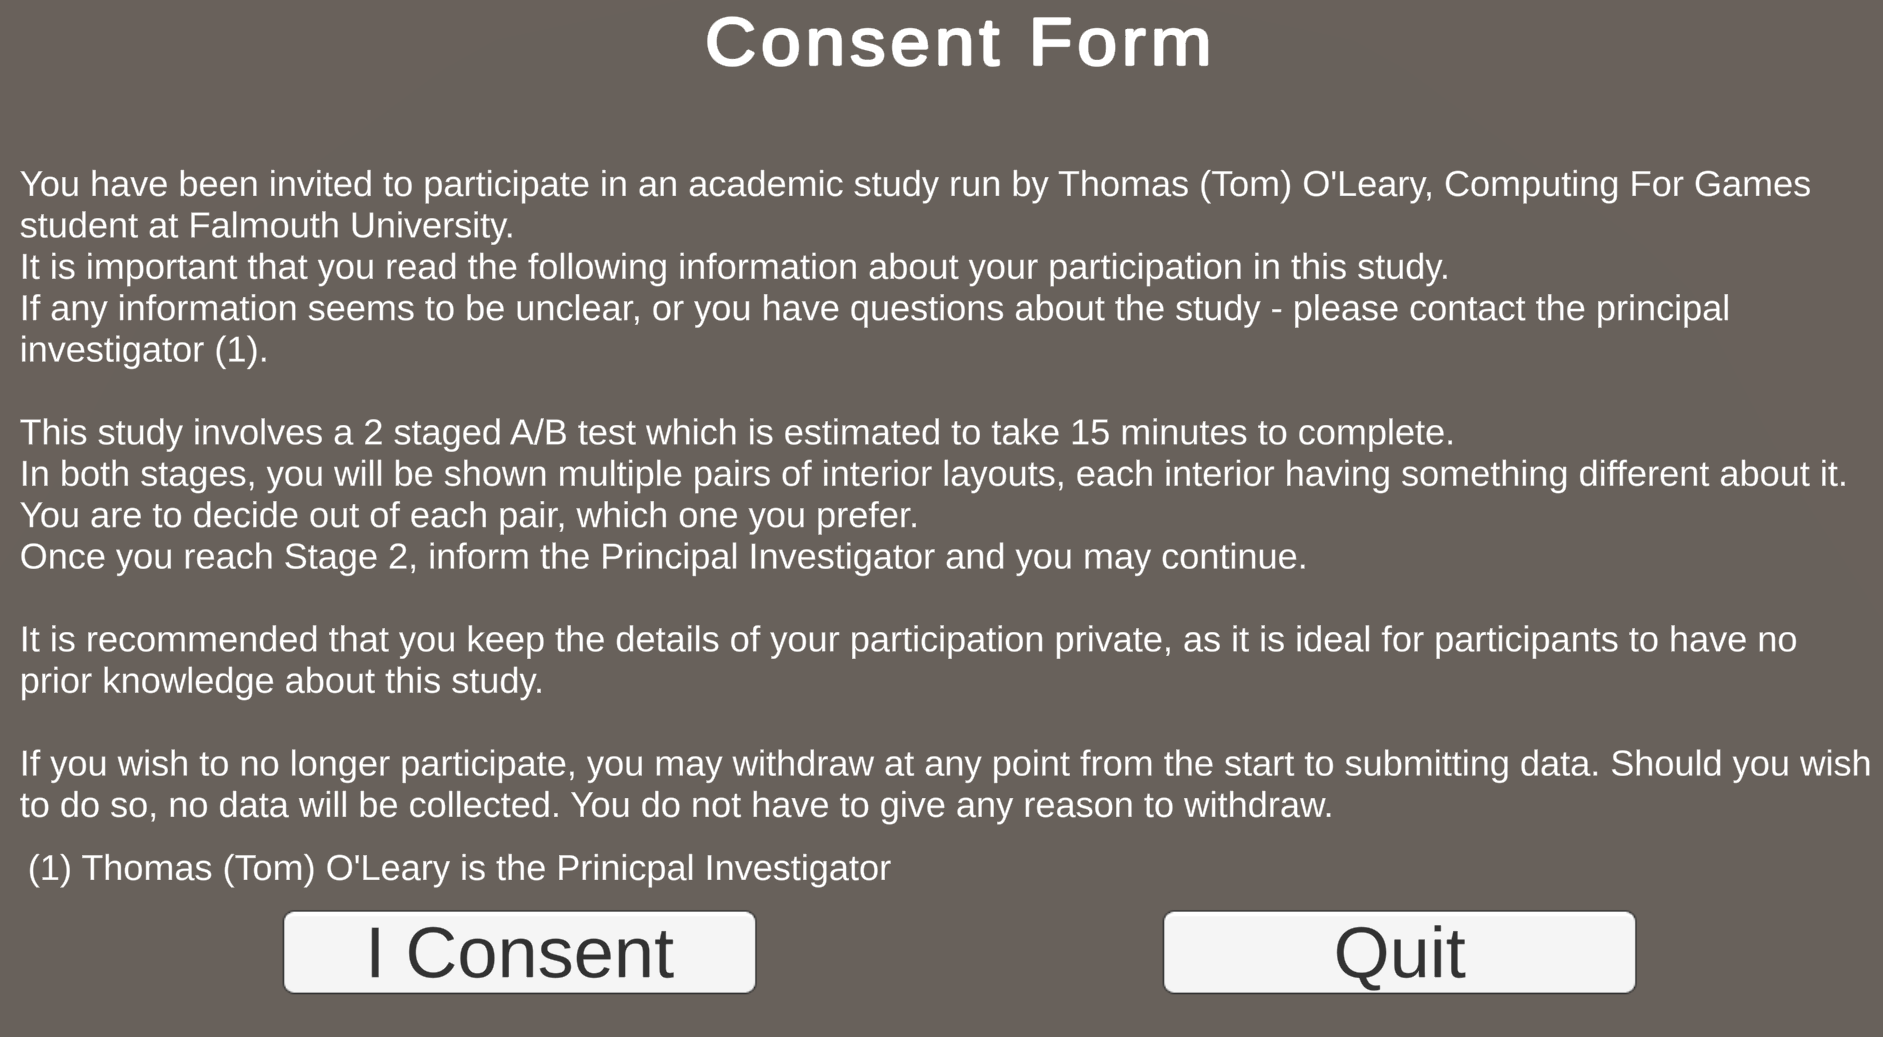
\includegraphics[width=\columnwidth]{./Images/consent-form.png}
    \centering
    \caption{The consent page before the start of the A/B test that the participant reads.}
    \label{consent-screen}
\end{figure}
\begin{figure}[!h]
    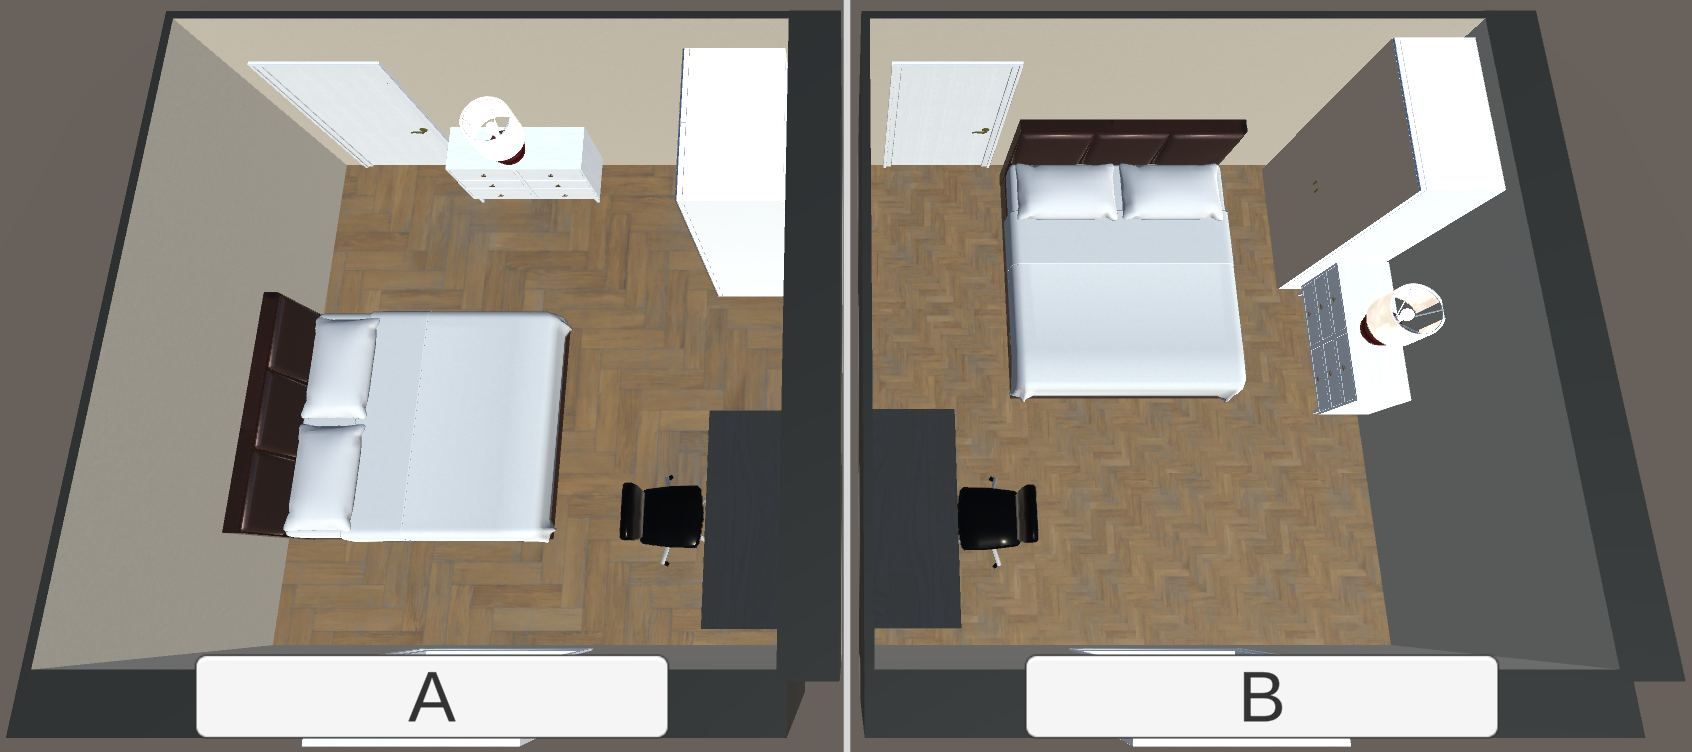
\includegraphics[width=\columnwidth]{./Images/pair-3.png}
    \centering
    \caption{A pair of furniture layouts used in the Research Study. One being human designed and the other being Artefact designed.}
    \label{pair-example-1}
\end{figure}
\begin{figure}[!h]
    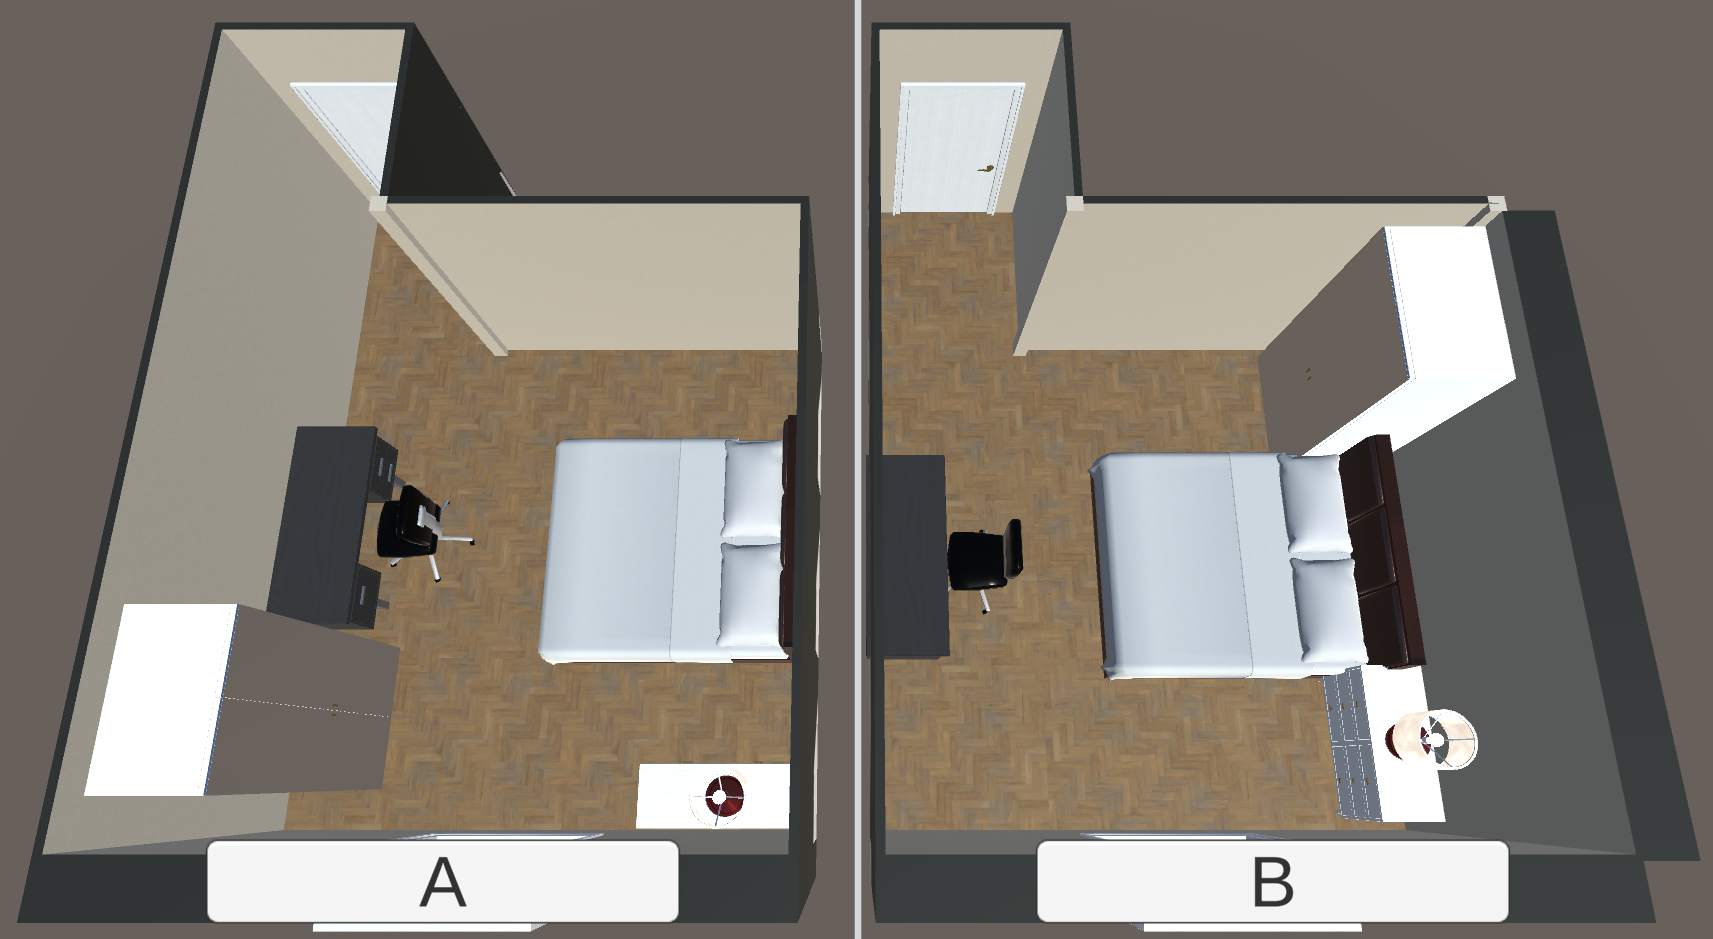
\includegraphics[width=\columnwidth]{./Images/pair-1.png}
    \centering
    \caption{Another pair that is used in the Research Study.}
    \label{pair-example-2}
\end{figure}
\begin{figure}[!h]
    
\includegraphics[width=\columnwidth]{./Images/stage-2-notice.png}
    \centering
    \caption{Screenshot of the Stage 2 notice, where participants are notified of the involvement of the Artefact.}
    \label{stage-2}
\end{figure}


\subsection{Sampling Plan}
To help answer my Hypotheses, I will be using two tailed T-Tests to allow me to easily identify the relationship between the selection of Human and Artefact designed layouts.
Using G*Power \cite{gpower}, I was able to calculate a sample size of 54 with an effect size of 0.5 - see Fig~\ref{gpower}.

\subsection{Data management plan}
As explained in Section \hyperref[ethics]{E}, no personal information is collected in the research study, nor can any information collected in the research study can be used to identify participants - signifying that General Data Protection Regulation (GDPR) \cite{gdpr} does not need to be followed. Results collected from the study however were exported and stored in a CSV file - see Fig~\ref{csv-file}. This file was password encrypted to prevent any third party intervention.


\subsection{Data Analysis}
Once sufficient data was collected from the research study, I used the R language and R-Studio for my analysis. In the code sample listed in \hyperref[append:b]{Appendix B}, I have demonstrated how to complete a Two Tailed T-Test using data from an imported CSV file.

\subsection{Ethical Considerations}\label{ethics}
As the research study requires human participants this creates a medium ethics risk according to the Falmouth University Ethics Board. To facilitate this risk, a Falmouth University ethics form was completed and signed off by the project Supervisor in consultation with the Head of Subject. The artefact itself is of low risk/concern as it is not used for militarization and participants are able to opt out at any point during their participation.
No personal information about the participants involved is collected nor can any data collected in the research study be used to identify participants - the EU's General Data Protection Regulation (GDPR)\cite{gdpr} does not need to be followed due to the nature of the research study. However, to protect the participants rights, the Nuremberg Code will be followed to keep and ensure this research study is ethically sound\cite{nuremberg-code}. All participants will be handed a Participant Information Sheet that details the key information they must know before the study, a consent form is also supplied to ensure they have agreed to participate. Participants are still able to withdraw at any point until submitting data.
\\
\subsubsection*{COVID-19}
At the current state of the pandemic and following the latest Government Guidelines in England \cite{gov-guidlines}, participants were not required to wear a face covering however they would not be questioned if they preferred to do so. All surfaces were sanitised between participants.
\\
\subsubsection*{Computer Related Injuries}
Due to the nature of the study taking place on a Computer, all forms of computer related injuries were taken into account. Participants had the opportunity to appropriately set the computers screen and seat positioning to the best ergonomic setting for themselves before starting the study. Participants were also informed that they could take a short break whenever they pleased.

\bibliographystyle{IEEEtran}
\bibliography{bibliography,bibliography2}

% Appendix
\section*{Appendix A - General} \label{append:a}
Link to the Ethics form and Participant Information Sheet:

\url{https://falmouthac-my.sharepoint.com/:f:/g/personal/to231922_falmouth_ac_uk/EiE3vOcxqLlLuU0_BN7m1NoBCja231kbqKHAxOlqX-sRfw?e=4dc65R}
\\
\\
Link to the Computing Artefact GitHub repository: 
\url{https://github.falmouth.ac.uk/TO231922/computing-artefact}
\begin{figure}[ht]
    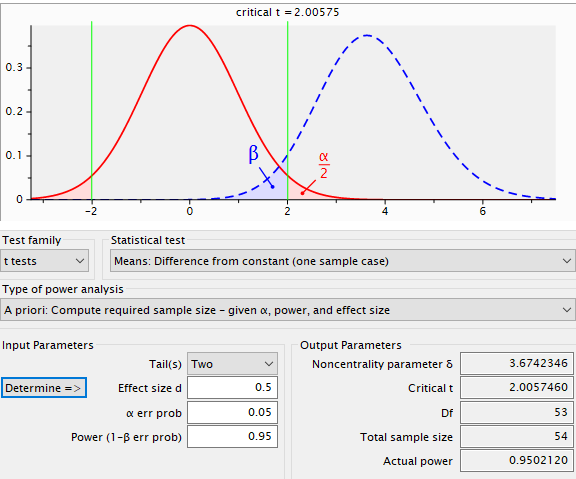
\includegraphics[width=\columnwidth]{./Images/gpower.png}
    \centering
    \caption{G*Power Sample Size}
    \label{gpower}
\end{figure}

\section*{Appendix B - Reflective Addendum} \label{append:b}


\newpage
\section*{Appendix C - Software Architecture} \label{append:c}
\begin{figure}[!h]
    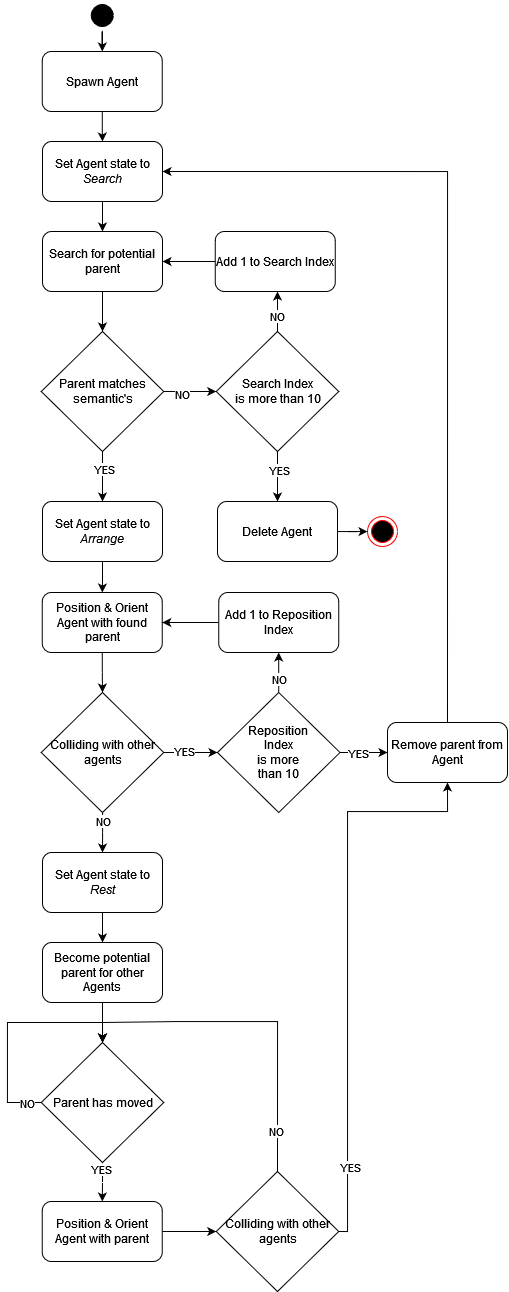
\includegraphics[width=\columnwidth]{./Images/AgentActivityDiagram.png}
    \centering
    \caption{Agent Behaviour represented in an Activity Diagram}
    \label{activity-diagram}
\end{figure}

\newpage
\section*{Appendix D - Testing} \label{append:d}
The Unit tests for my artefact were created using Unity's Test Framework and were used throughout the Artefact's development to validate the code and to ensure the Artefact worked as intended. Unit testing code can be seen in \hyperref[append:f]{Appendix F} and passed Unit Tests can be seen in Fig~\ref{unit-tests}.
\\
A small pilot study was conducted with the help of some BSc peers. This pilot study was conducted to ensure the validity of my experimental design. It consisted of them taking part in my 2-staged A/B test, helping in testing the effectiveness of how information was being represented - any feedback received from this small study was implemented into my methodology and no data from this pilot study was used within my data analysis.

\begin{figure}[ht]
    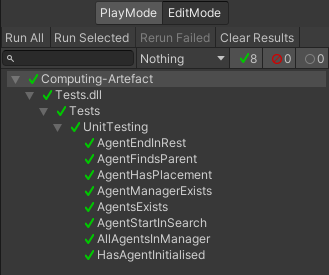
\includegraphics[width=\columnwidth]{./Images/unit-tests.png}
    \centering
    \caption{Unit Tests in the Unity Test Runner}
    \label{unit-tests}
\end{figure}

\newpage
\newpage
\section*{Appendix E - R Code} \label{append:e}
\lstinputlisting[language=r, label=StageOneRCode,caption=R Code for Stage One data., captionpos=b]{Code/StageOneRCode.R}

\lstinputlisting[language=r, label=StageTwoRCode,caption=R Code for Stage Two data., captionpos=b]{Code/StageTwoRCode.R}

\newpage
\section*{Appendix F - Unit Testing Code} \label{append:f}
\lstinputlisting[language=csh, label=UnitTestCode, caption=Unit Test Code used to validate the Artefact's code., captionpos =b]{Code/UnitTesting.cs}

\end{document}